\chapter{CIDR Report Analysis and Observations}
\label{chap:analysis}

\section{Characteristics of the CIDR Report}

\begin{figure}
    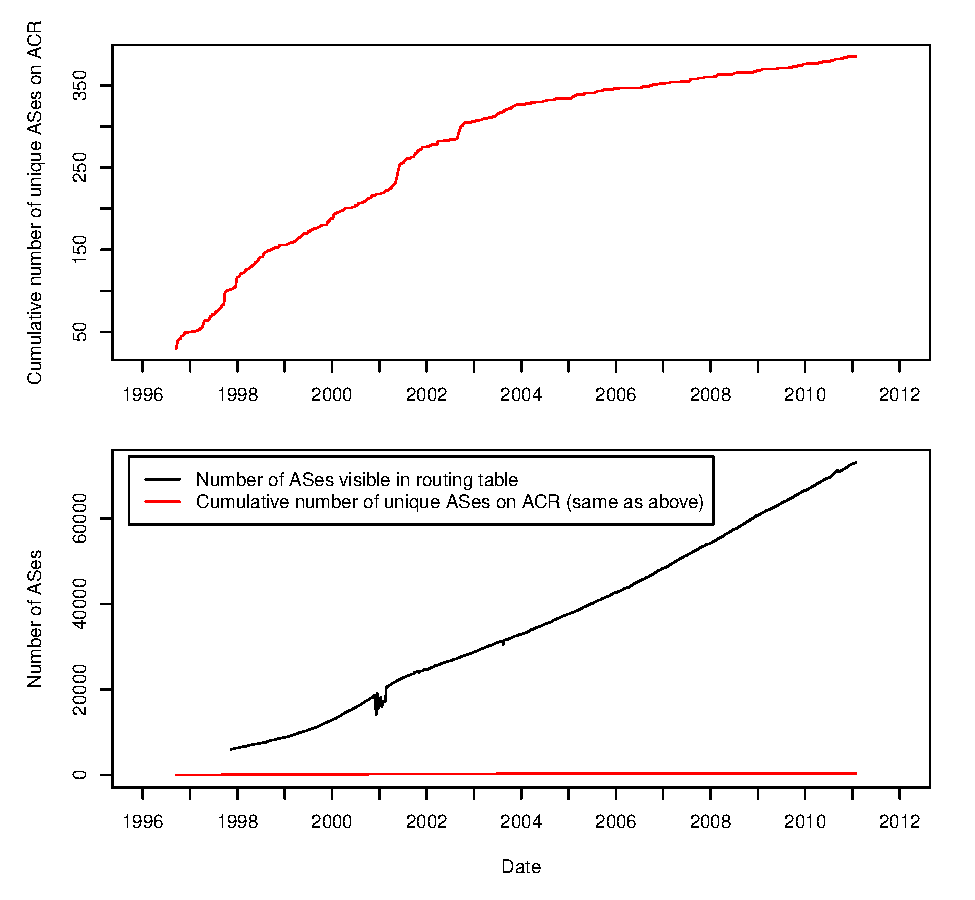
\includegraphics[width=6in]{figures/cumulative_asn_counts.pdf}
    \caption{A cumulative count of the unique ASes that have appeared on the CIDR Report and compared to the unique ASes visible in the routing table at the same moment.}
\end{figure}

\begin{figure}
    \includegraphics[width=6in]{figures/viz_sample.jpg}
    \caption{Visualization sample.}
\end{figure}

\section{Analysis of AS behavior after appearing on the CIDR Report}

blah blah blah blah

\begin{figure}
    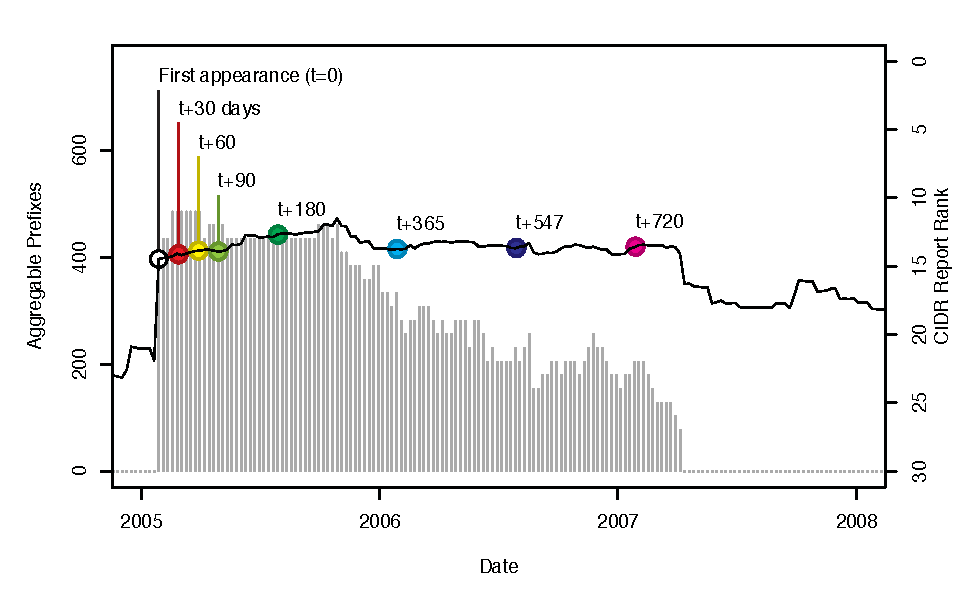
\includegraphics[width=6in]{figures/single_as.pdf}
    \caption{Measurement methodology explanation (AS 3602).}
\end{figure}


\subsection{Implementation Accuracy}

blah blah blah blah

\begin{figure}
    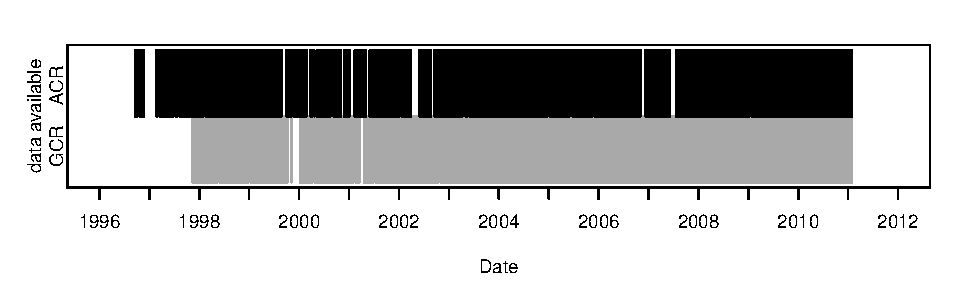
\includegraphics[width=6in]{figures/data_avail.pdf}
    \caption{Available data}
\end{figure}

\begin{figure}
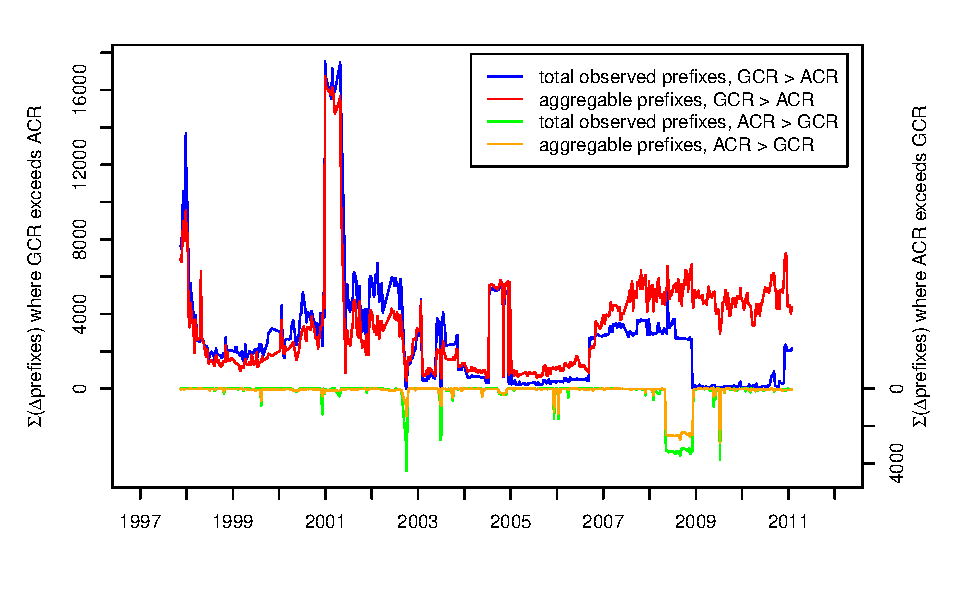
\includegraphics[width=6in]{figures/cidr_report_validity_prefix_error.pdf}
    \caption{Differences in prefix counts between authoritative (ACR) and generated (GCR) CIDR Reports over time.}
\end{figure}

\begin{figure}
    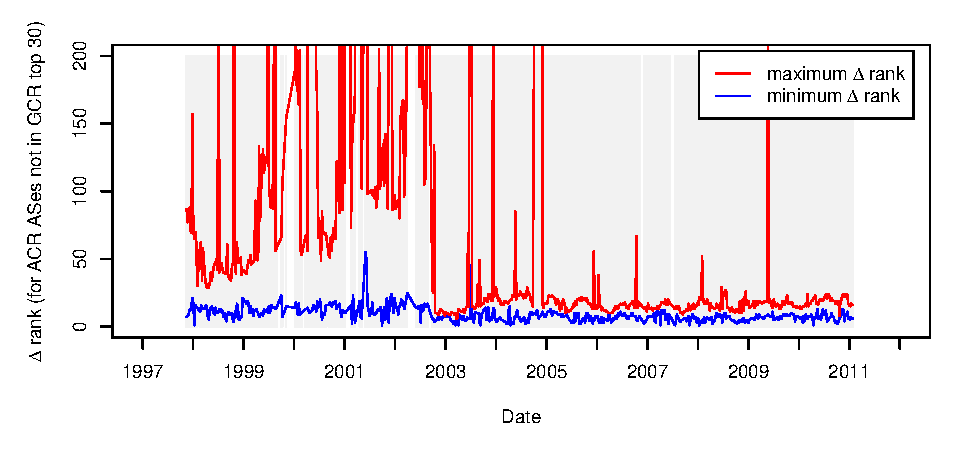
\includegraphics[width=6in]{figures/cidr_report_validity_rank_error.pdf}
    \caption{Minimum and maximum differences in ASes ranked in the top 30 on the ACR but not in the top 30 on the GCR.}
\end{figure}

\begin{figure}
    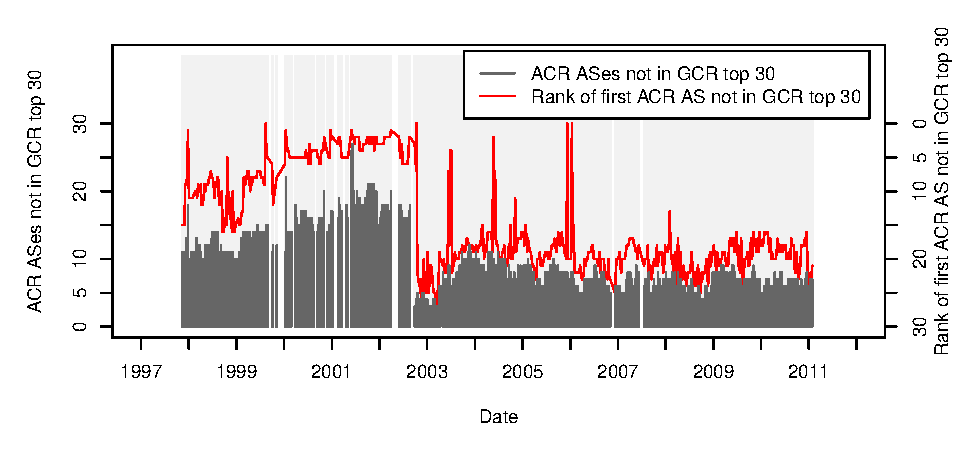
\includegraphics[width=6in]{figures/cidr_report_validity_top30_error.pdf}
    \caption{The number and first rank of ASes in the treatment group (top 30) of the ACR that are not in the treatment group of the GCR over time.}
\end{figure}

\fbox{plot deaggregation factor too -- 1 / (1 - aggfrac) or total/(total-aggregable)!!}

\subsection{Interpretation}

In spite of seeing aggregation behavior relative to the control, the total number of routes in the routing table does not drop over time, suggesting that old people are replaced by new ``bad guys'' or new entrants. Cittadini's study suggests that the proportion of ``bad guys'' remains the same over time (the people that would show up on the CIDR Report), suggesting the rolling-over bad guy theory.

OR. The table just grew less quickly than it otherwise could have, but we can't examine the counterfactual world...?

Rolling-over bad guy theory would be supported by the rate of growth of new ASes on teh CIDR report?

Arthur suggests looking at the fraction (# of /24s / # of prefixes in the routing table) per AS or for the entire routing table, over time

What do Cittadini's observations mean for my analysis of the later repport where people are far more deaggregated

\subsection{Validity}
It was an oversight that I didn't measure behavior of ASes before their appearance on the CIDR Reprot. However, because appearance is determined based on netgain behavior means this is likely as not as huge a challenge to validity as I expected. I still need to be concerned that appearance didn't occur because someone else got less bad, but in such a case one's aggregation fraction would be at best flat, not decreasing to start (or they should've appeared earlier).



%ANALYSIS
%
%- Available data/data overview
%	- plot 'h' plots of available data
%	- plot total prefixes in the total table (Routeviews) and in the report (Cidr Report) to see that there aren't any discontinuities
%
%- Accuracy/error of my implementation of the CIDR report
%
%- Visualization of aggregate behavior and general characteristics (in particular stratification at the top of the CIDR report)
%    - Definition of metrics used in the analysis
%        - rank on CIDR Report (order by netgain)
%        - absolute/delta netgain
%        - relative/delta netgain (relative to netsnow)
%    - CDFs by AS appearnace
%    - CDFs by rank
%
%    - Summary/general statistics and characteristics of behavior over time (time series?), across and within groups, etc. (p62)
%
%- AS Behavior after appearing on the CIDR Report
%	- Distribution of AS behaviors from T=0, T=+1 month, 3 m, 6m, 1y, 2y, etc.
%		- all appearances on the cidr report
%		- no appearance/randomly selected control
%		- appearances that actually had behavior changes observed
%	- slice by date (NOT by rank on CIDR report), and by netsnow
%
%- Variance in views of data from different peers
%- for different origin ASes that appear on the CIDR Report
%- across the entire routing table
%
%////////////////////////////////////////////////////////////////////////////////
%////////////////////////////////////////////////////////////////////////////////
%////////////////////////////////////////////////////////////////////////////////
%
%DISCUSSION
%
%Discussion of the design assumptions, and the sensitivity of the CIDR report to those assumptions
